% REST resource map of /api/v1 -- replaces the Swagger screenshots (Section 3.2).
\documentclass[tikz,border=1pt]{standalone}
% =====================================================================
%  Shared style for every diagram in the proposal.
%  Each figure is a standalone TikZ file that \input's this preamble, so
%  all diagrams use the same font family (Computer Modern, T1 -- identical
%  to the LLNCS body text), the same sizes and the same palette.
%
%  Font rule (do not change per figure):
%    node text   \footnotesize  (8 pt)
%    edge labels \scriptsize    (7 pt)
%    titles      \footnotesize\bfseries
%  Figures are drawn at their final width (<= 12.2 cm, the LLNCS text
%  width) and included WITHOUT scaling, so the printed size is the same
%  in every figure.
% =====================================================================
\usepackage[T1]{fontenc}
\usepackage{amsmath,amssymb}
\usepackage{xcolor}
\usepackage{tikz}
\usetikzlibrary{positioning,arrows.meta,shapes.geometric,shapes.multipart,
  fit,backgrounds,calc,shadows,patterns}

% ---- palette ---------------------------------------------------------
\definecolor{cBlue}{HTML}{0B4F8A}    % application / API
\definecolor{cOrange}{HTML}{B4540A}  % processing / services
\definecolor{cPurple}{HTML}{5B3CC4}  % data stores
\definecolor{cGreen}{HTML}{1B7A3A}   % success / output
\definecolor{cRed}{HTML}{B42318}     % error / risk
\definecolor{cGray}{HTML}{5F6672}    % external / neutral
\definecolor{cInk}{HTML}{1F2933}     % text and arrows

\colorlet{fBlue}{cBlue!9}
\colorlet{fOrange}{cOrange!10}
\colorlet{fPurple}{cPurple!9}
\colorlet{fGreen}{cGreen!10}
\colorlet{fRed}{cRed!9}
\colorlet{fGray}{cGray!8}

% ---- fonts -----------------------------------------------------------
\newcommand{\figfont}{\footnotesize}
\newcommand{\lblfont}{\scriptsize}
\newcommand{\code}[1]{\texttt{#1}}

\tikzset{
  every picture/.style={font=\figfont, line join=round, >={Stealth[length=4pt,width=3.4pt]}},
  every node/.append style={execute at begin node={\hyphenpenalty=10000\exhyphenpenalty=10000}},
  base/.style={draw, rounded corners=2pt, line width=0.6pt, align=center,
               inner xsep=3pt, inner ysep=2.5pt, text=cInk, font=\figfont},
  app/.style={base, draw=cBlue, fill=fBlue},
  svc/.style={base, draw=cOrange, fill=fOrange},
  data/.style={base, draw=cPurple, fill=fPurple},
  ok/.style={base, draw=cGreen, fill=fGreen},
  bad/.style={base, draw=cRed, fill=fRed},
  ext/.style={base, draw=cGray, fill=fGray},
  plain/.style={base, draw=none, fill=none},
  db/.style={cylinder, shape border rotate=90, aspect=0.22, draw=cPurple,
             fill=fPurple, line width=0.6pt, align=center, text=cInk,
             minimum height=9mm, font=\figfont},
  decision/.style={diamond, aspect=2.2, draw=cOrange, fill=fOrange,
                   line width=0.6pt, align=center, inner sep=1pt, text=cInk, font=\figfont},
  actor/.style={draw=cInk, fill=fGray, line width=0.8pt, rounded corners=0pt,
                align=center, inner sep=3pt, font=\figfont\bfseries},
  layer/.style={draw=cGray!60, fill=cGray!4, rounded corners=3pt, line width=0.5pt},
  layertitle/.style={font=\lblfont\bfseries, text=cGray, anchor=north west, inner sep=2pt},
  arr/.style={->, draw=cInk, line width=0.6pt},
  darr/.style={->, draw=cGray, line width=0.6pt, dashed},
  biarr/.style={<->, draw=cInk, line width=0.6pt},
  lbl/.style={font=\lblfont, text=cInk, inner sep=1.5pt},
  lblbg/.style={font=\lblfont, text=cInk, inner sep=1.5pt, fill=white},
}

% ---- UML sequence-diagram helpers -----------------------------------
%  \lifeline{id}{x}{label}{bottom y}   head box + dashed life line
%  \msg{x1}{x2}{y}{label}              synchronous call (solid)
%  \ret{x1}{x2}{y}{label}              reply (dashed)
%  \selfmsg{x}{y}{label}               call to self, label on the right
%  \fragment{kind}{guard}{x1}{y1}{x2}{y2}  combined fragment (alt/loop/par)
\newcommand{\lifeline}[4]{%
  \node[app, text width=19mm, minimum height=8.5mm, font=\figfont\bfseries] (#1) at (#2,0) {#3};
  \draw[cGray, dashed, line width=0.5pt] (#1.south) -- (#2,#4);}
\newcommand{\msg}[4]{%
  \draw[arr] (#1,#3) -- node[lbl, above] {#4} (#2,#3);}
\newcommand{\ret}[4]{%
  \draw[darr] (#1,#3) -- node[lbl, above] {#4} (#2,#3);}
\newcommand{\selfmsg}[3]{%
  \draw[arr] (#1,#2+0.12) -- ++(0.3,0) -- ++(0,-0.24) -- ++(-0.3,0);
  \node[lbl, anchor=west, align=left] at (#1+0.35,#2) {#3};}
\newcommand{\fragment}[6]{%
  \draw[cGray, line width=0.5pt] (#3,#4) rectangle (#5,#6);
  \node[anchor=north west, draw=cGray, fill=white, font=\lblfont\bfseries,
        inner sep=1.5pt, line width=0.5pt] at (#3,#4) {#1};
  \if\relax\detokenize{#2}\relax\else
  \node[anchor=north west, font=\lblfont, text=cGray, inner sep=1.5pt] at (#3+0.75,#4) {[#2]};\fi}
\newcommand{\activation}[3]{% x, y top, y bottom
  \draw[draw=cBlue, fill=fBlue, line width=0.5pt] (#1-0.07,#2) rectangle (#1+0.07,#3);}

\usepackage{array}
\setlength{\fboxsep}{0.9pt}
\setlength{\fboxrule}{0.5pt}
\newcommand{\badge}[3]{\fcolorbox{#1}{#2}{\makebox[9.5mm]{\ttfamily\scriptsize\bfseries\color{#1}#3}}}
\newcommand{\GET}{\badge{cGreen}{fGreen}{GET}}
\newcommand{\POST}{\badge{cBlue}{fBlue}{POST}}
\newcommand{\PUT}{\badge{cOrange}{fOrange}{PUT}}
\newcommand{\DEL}{\badge{cRed}{fRed}{DELETE}}
\newcommand{\st}[1]{\textcolor{cGray}{\ttfamily #1}}
\newenvironment{ops}{\renewcommand{\arraystretch}{1.12}\setlength{\tabcolsep}{2.5pt}%
  \begin{tabular}{@{}l >{\ttfamily}p{41mm} >{\raggedright\arraybackslash}p{33mm} r@{}}}{\end{tabular}}
\tikzset{grp/.style={base, draw=cBlue, fill=white, align=left, inner sep=3pt, anchor=north west}}
\begin{document}
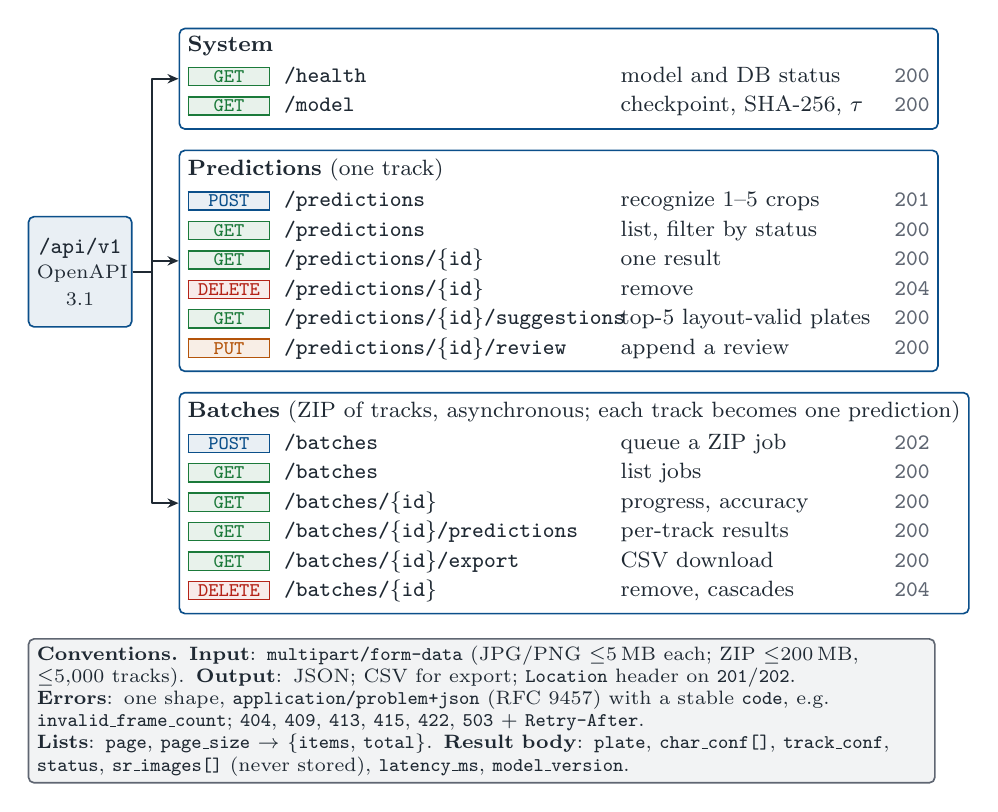
\begin{tikzpicture}
  \node[app, minimum height=14mm, text width=11mm] (root) at (0.75,-3.1) {\code{/api/v1}\\[1pt]\lblfont OpenAPI\\\lblfont 3.1};

  \node[grp] (sys) at (2.0,0) {\textbf{System}\\[1pt]
    \begin{ops}
      \GET & /health & model and DB status & \st{200} \\
      \GET & /model  & checkpoint, SHA-256, $\tau$ & \st{200} \\
    \end{ops}};
  \node[grp, below=2.5mm of sys.south west, anchor=north west] (pre) {\textbf{Predictions} (one track)\\[1pt]
    \begin{ops}
      \POST & /predictions & recognize 1--5 crops & \st{201} \\
      \GET  & /predictions & list, filter by status & \st{200} \\
      \GET  & /predictions/\{id\} & one result & \st{200} \\
      \DEL  & /predictions/\{id\} & remove & \st{204} \\
      \GET  & /predictions/\{id\}/suggestions & top-5 layout-valid plates & \st{200} \\
      \PUT  & /predictions/\{id\}/review & append a review & \st{200} \\
    \end{ops}};
  \node[grp, below=2.5mm of pre.south west, anchor=north west] (bat) {\textbf{Batches} (ZIP of tracks, asynchronous; each track becomes one prediction)\\[1pt]
    \begin{ops}
      \POST & /batches & queue a ZIP job & \st{202} \\
      \GET  & /batches & list jobs & \st{200} \\
      \GET  & /batches/\{id\} & progress, accuracy & \st{200} \\
      \GET  & /batches/\{id\}/predictions & per-track results & \st{200} \\
      \GET  & /batches/\{id\}/export & CSV download & \st{200} \\
      \DEL  & /batches/\{id\} & remove, cascades & \st{204} \\
    \end{ops}};

  \foreach \g in {sys,pre,bat} \draw[arr] (root.east) -- ++(0.25,0) |- (\g.west);

  % conventions
  \node[base, draw=cGray, fill=fGray, align=left, text width=113mm, anchor=north west, font=\lblfont]
    (conv) at ([yshift=-3mm]root.west |- bat.south) {%
    \textbf{Conventions.}
    \textbf{Input}: \code{multipart/form-data} (JPG/PNG $\le$5\,MB each; ZIP $\le$200\,MB, $\le$5{,}000 tracks).
    \textbf{Output}: JSON; CSV for export; \code{Location} header on \code{201}/\code{202}.\\
    \textbf{Errors}: one shape, \code{application/problem+json} (RFC 9457) with a stable \code{code}, e.g.\ \code{invalid\_frame\_count};
    \code{404}, \code{409}, \code{413}, \code{415}, \code{422}, \code{503} + \code{Retry-After}.\\
    \textbf{Lists}: \code{page}, \code{page\_size} $\rightarrow$ \{\code{items}, \code{total}\}.
    \textbf{Result body}: \code{plate}, \code{char\_conf[]}, \code{track\_conf}, \code{status}, \code{sr\_images[]} (never stored), \code{latency\_ms}, \code{model\_version}.};
\end{tikzpicture}
\end{document}
